\documentclass[twocolumn]{article}

\usepackage{geometry}
\geometry{textwidth = 18cm,textheight = 24cm}

\usepackage{cite}
\usepackage{caption}
\usepackage{graphicx}
\usepackage{amsmath}
\usepackage{amssymb}
%\usepackage{braket}
\usepackage{textcomp}
%\usepackage{lmodern}
\usepackage{authblk}
\usepackage{datetime}
\usepackage{gensymb}
\usepackage{wrapfig}
%\usepackage[usenames,dvipsnames,svgnames,table]{xcolor}
\usepackage{booktabs}
%\usepackage{appendix}

%\usepackage[switch,columnwise]{lineno}
%\linenumbers

\newcommand{\onlinecite}[1]{\hspace{-1 ex} \nocite{#1}\citenum{#1}} 

\let\OLDthebibliography\thebibliography
\renewcommand\thebibliography[1]{
  \OLDthebibliography{#1}
  \setlength{\parskip}{0pt}
  \setlength{\itemsep}{0pt plus 0.3ex}
}
  
\title{Modeling Loop Neurons as Systems of Leaky Integrators}
\author[1]{\Large{NIST Physics and Hardware for Intelligence Project}
\\
\textit{\large{National Institute of Standards and Technology}}
\\
\vspace{-0.2em}
\textit{\large{325 Broadway, Boulder, CO, USA, 80305}}
\\
\vspace{-0.2em}
\textit{\large{jeffrey.shainline@nist.gov}}
}
\date{\today}%\today

\begin{document}

\twocolumn[
  \begin{@twocolumnfalse}
    \maketitle
    \begin{abstract}

    \vspace{3em}
    \end{abstract}
  \end{@twocolumnfalse}
]

\setcounter{tocdepth}{1}
\setcounter{secnumdepth}{4}
\tableofcontents

\section{\label{sec:introduction}Introduction}

\begin{figure}[h!]
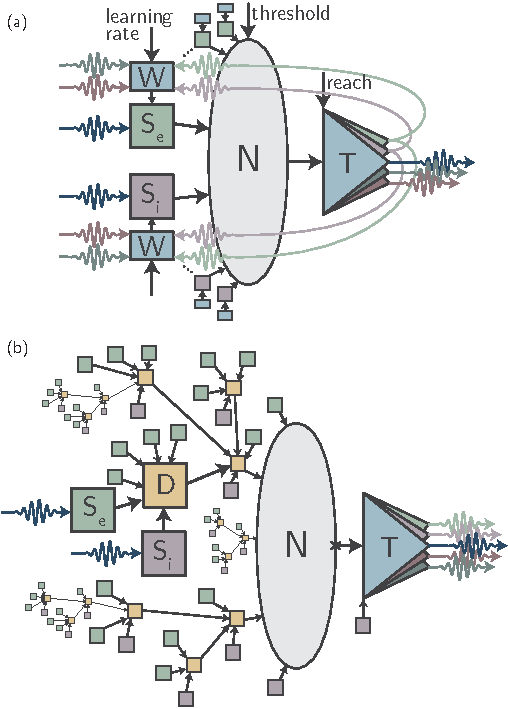
\includegraphics[width=8.6cm]{figures/_fig__schematics.pdf}
\captionof{figure}{\label{fig:schematic__circuits}Two schematics of loop neurons. (a) Schematic of point neuron. (b) Schematic of neuron with dendritic tree.}
\end{figure}

\begin{equation}
\label{eq:leaky_integrator}
\frac{dV(t)}{dt} = f(t)-\frac{V(t)}{\tau},
\end{equation}


\section{\label{sec:synapses}Synapses}


This description of the operation of the circuit is based on well-known properties of Josephson junctions within the formalism of the resistively and capacitively shunted junction (RCSJ) model \cite{vatu1998,ka1999,ti1996}. The relevant behavior derives from the fact that a JJ will produce a voltage fluxon after a time $t_{\mathrm{fq}}$ determined by the relation
\begin{equation}
\label{eq:jj__fluxon_production}
\int_0^{t^{\mathrm{fq}}}V(t)dt = \Phi_0.
\end{equation}
If $V(t)$ is slowly varying on the scale of $t^{\mathrm{fq}}$, we can make the approximation $V(t)\,t^{\mathrm{fq}} \approx \Phi_0$, giving the rate of fluxon generation as
\begin{equation}
\label{eq:jj__fluxon_rate}
r^{\mathrm{fq}}(t) =  \frac{1}{t^{\mathrm{fq}}} = \frac{V(t)}{\Phi_0}.
\end{equation}

\begin{equation}
\label{eq:synapses__leaky_integrator}
\frac{dI^{\mathrm{si}}(t)}{dt} = I^{\mathrm{fq}}\,r^{\mathrm{fq}}\left(I^{(\mathrm{sf})}(t),I^{(\mathrm{si})}(t)\right) -\frac{I^{(\mathrm{si})}(t)}{\tau^{(\mathrm{si})}},
\end{equation}
where the function $r^{\mathrm{fq}}\left(I^{(\mathrm{sf})},I^{(\mathrm{si})}\right)$ represents the rate at which fluxons are added to the SI loop as a function of the total current across the synaptic firing junction, $I^{\mathrm{sf}}$, as well the current circulating in the SI loop, $I^{\mathrm{si}}$. $I^{\mathrm{fq}} = \Phi_0/L^{\mathrm{si}}$ is the current added to the SI loop with each fluxon. The flux-induced current $I^{\mathrm{si}}$ circulates in the SI loop in a manner that counters the bias to $J^{\mathrm{si}}$. It is this counter-biasing that causes the SI loop to saturate as a function of $I^{\mathrm{si}}$. When $I^{\mathrm{si}}$ becomes sufficiently large, the fluxon generated by $J^{\mathrm{jtl}}$ does not provide enough current to drive $J^{\mathrm{si}}$ above $I_c$, and the stored flux in the SI loop must decay before subsequent synapse events can add to the integrated signal.

\begin{equation}
\label{eq:jj__current_voltage}
V^{\mathrm{sf}}(I^{\mathrm{sf}}) = \begin{cases} V_0\left[ \left( \frac{I^{\mathrm{sf}}}{I_c-I_r} \right)^{\mu_1} - 1 \right]^{\mu_2}, & \text{for } I > (I_c-I_r)_+ \\
0, & \text{for } I < (I_c)_-
\end{cases}
\end{equation} 
where the values $\mu_1$, $\mu_2$, and $V_0$ depend on the specific parameters of the shunt resistance and capacitance in the RCSJ model. For the junctions considered here, $I_r = 1.1768$\,\textmu A is the reset current associated with hysteresis on $J_{\mathrm{sf}}$ due to the fact that $\beta_c = 0.95 > 0$. $\mu_1 = 3.464271$, $\mu_2 = 0.306768$, and $V_0 = 233.966$\,\textmu V. From Eqs.\,\ref{eq:jj__fluxon_production} and \ref{eq:jj__current_voltage} we can obtain $r^{\mathrm{fq}}$. In the case where $I^{(\mathrm{sf})}$ is slowly varying compared to $t^fq$, $ r^{\mathrm{fq}} = V^{(\mathrm{sf})}/\Phi_0$. The notation $I > (I_c-I_r)_+$ refers to currents $I$ that have exceeded $I_c$, driving the junction into the resistive state, and have yet to drop below $I_c-I_r$, and are therefore demonstrating hysteresis. Likewise, $I<(I_c)_-$ refers to currents that are below $I_c$ while the junction is not in the hysteretic state.


\begin{figure}[h!]
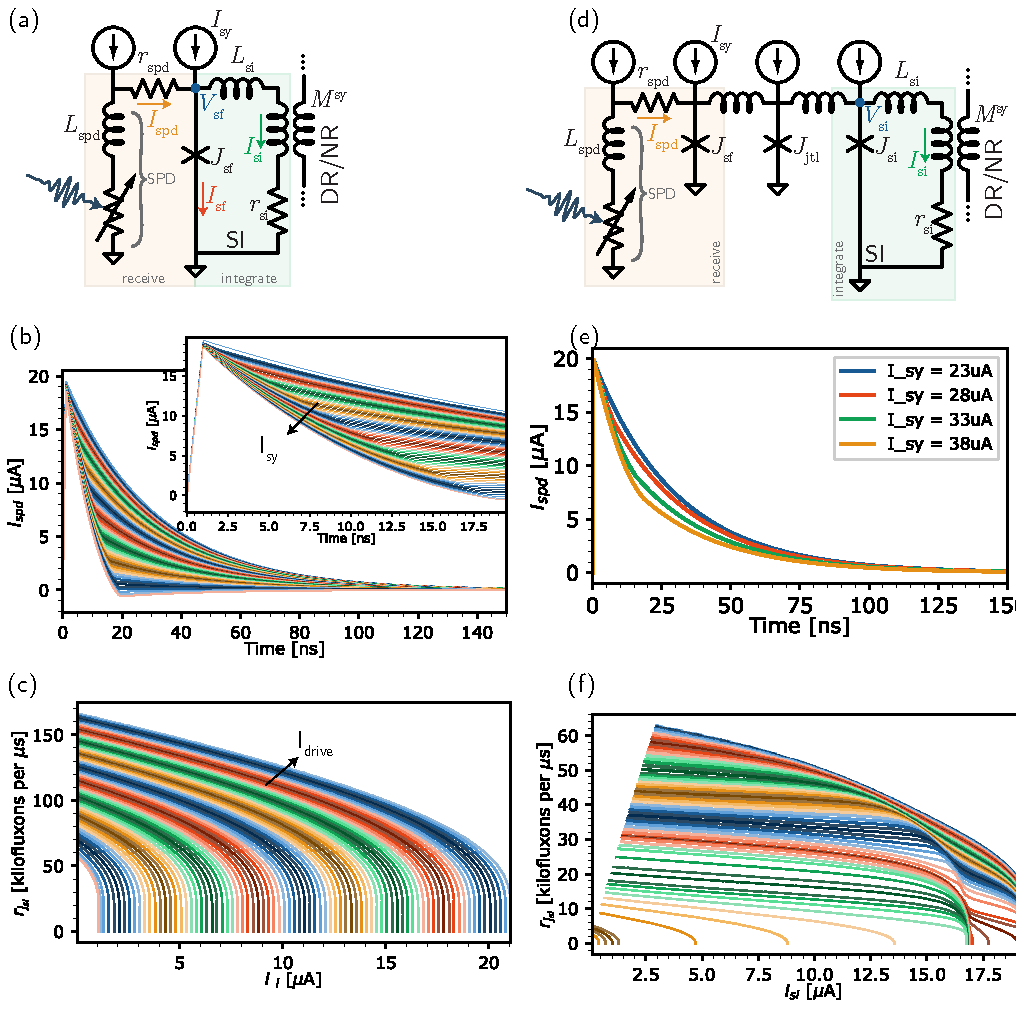
\includegraphics[width=8.6cm]{figures/_fig__synapses__circuits_responses.pdf}
\captionof{figure}{\label{fig:synapses__responses}Caption.}
\end{figure}

\begin{figure}[h!]
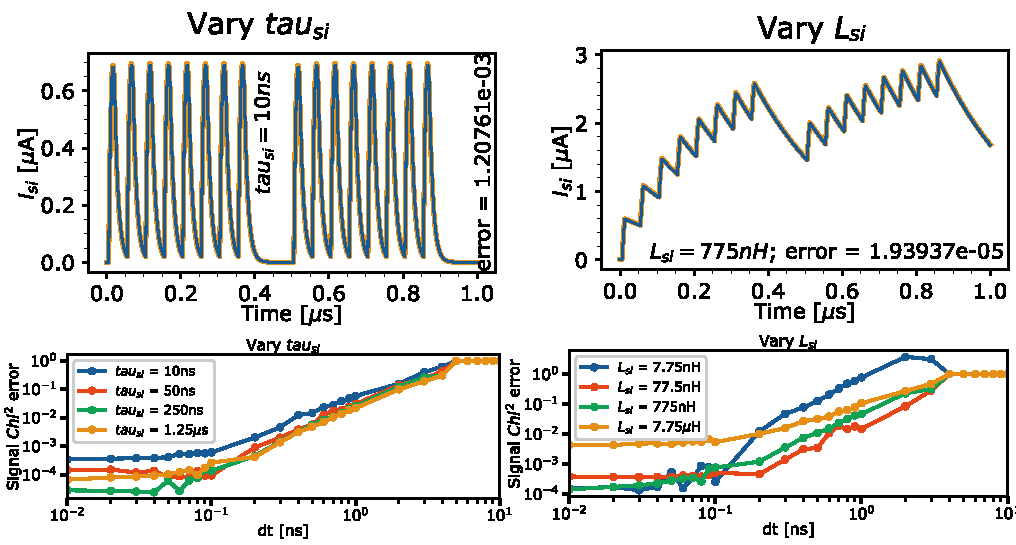
\includegraphics[width=8.6cm]{figures/_fig__synapses__comparison.pdf}
\captionof{figure}{\label{fig:synapses__comparison}Caption.}
\end{figure}


\section{\label{sec:dendrites}Dendrites}

\begin{equation}
\label{eq:dendrites__leaky_integrator}
\frac{dI^{(\mathrm{di})}(t)}{dt} = I^{\mathrm{fq}}\,r^{\mathrm{fq}} \left( \Phi^{(\mathrm{dr})}_a(t),I^{(\mathrm{di})}(t) \right) - \frac{I^{(\mathrm{di})}(t)}{\tau^{(\mathrm{di})}},
\end{equation}
where $\Phi^{(\mathrm{dr})}_a(t)$ is the total applied flux to the dendritic receiving loop:
\begin{equation}
\label{eq:dendrites__applied_flux}
\Phi^{(\mathrm{dr})}_a(t) = \sum_i M_i I_i^{(\mathrm{si/di})}(t).
\end{equation}
The sum runs over all inputs to the dendritic receiving loop, and the superscript notation $I_i^{(\mathrm{si/di})}$ indicates that inputs may be from synaptic or dendritic integration loops.

\begin{figure}[h!]

\includegraphics[width=8.6cm]{figures/_fig__dendrites__circuits_responses.pdf}
\captionof{figure}{\label{fig:dendrites__responses}Caption.}
\end{figure}

\begin{figure}[h!]

\includegraphics[width=8.6cm]{figures/_fig__dendrites__comparison.pdf}
\captionof{figure}{\label{fig:dendrites__comparison}Caption.}
\end{figure}


\section{\label{sec:neurons}Neurons}

\begin{figure}[h!]
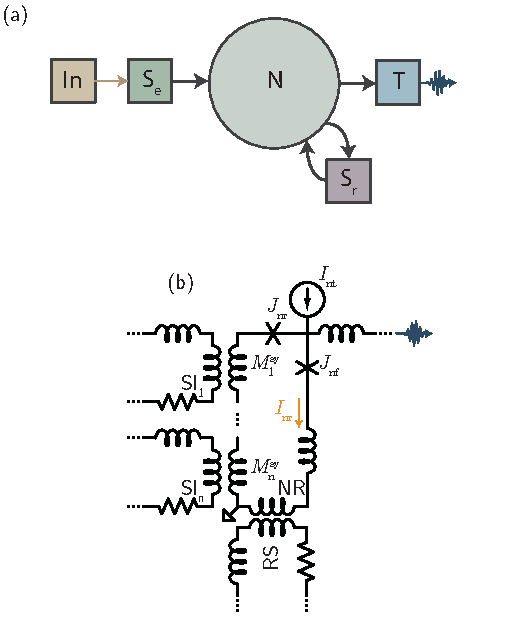
\includegraphics[width=8.6cm]{figures/_fig__point_neuron__schematic__circuit.pdf}
\captionof{figure}{\label{fig:point_neuron__schematic__circuit}Caption.}
\end{figure}

\section{\label{sec:discussion}Discussion}



\bibliographystyle{unsrt}
\bibliography{phenomenological_modeling}

\end{document}